\chapter{Numerical and Graphical Limits}

Solve using the graph of $f(x)$ below.	\newline\\

\begin{center}
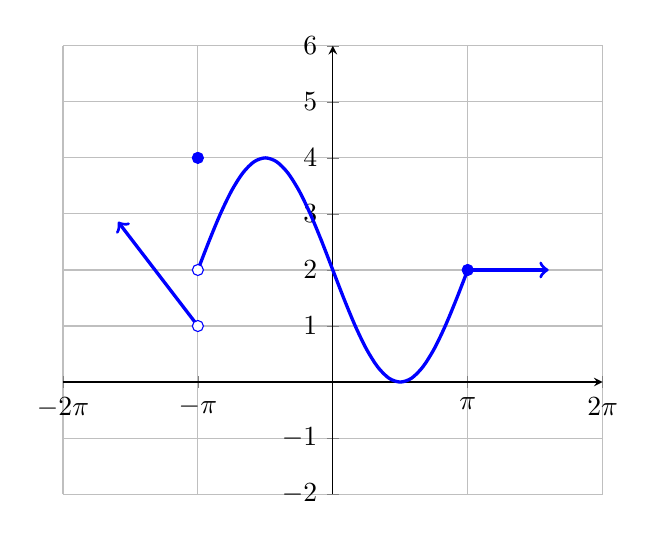
\begin{tikzpicture}
\begin{axis}[
axis lines = middle, xmin = -2*pi, xmax = 2*pi, xtick = {-2*pi, -pi, 0, pi, 2*pi}, xticklabels = {$-2\pi$, $-\pi$, , $\pi$, $2\pi$}, ymin = -2, ymax = 6, grid, ytick = {-2,-1,...,6}
]
\addplot[<-, very thick, blue, domain=-5:-pi] {-x-2.14};
\addplot[very thick, blue, domain=-pi:pi, smooth] {2*sin(deg(x+pi))+2};
\addplot[->, very thick, blue, domain=pi:1.6*pi] {2};
\addplot[blue, mark=*, only marks] coordinates {(-pi,4) (pi,2)};
\addplot[blue, fill=white, mark=*, only marks] coordinates {(-pi,1) (-pi,2)};
\end{axis}
\end{tikzpicture}
\end{center}

\begin{multicols}{4}
\begin{enumerate}   
    \item $\lim_{x \to -\pi^-}f(x)$
    \item $\lim_{x \to -\pi^+}f(x)$
    \item $\lim_{x \to -\pi}f(x)$
    \item $f(-\pi)$
    \item $\lim_{x \to \pi^-}f(x)$
    \item $\lim_{x \to \pi^+}f(x)$
    \item $\lim_{x \to \pi}f(x)$
    \item $f(\pi)$
\end{enumerate}     \setcounter{Review}{\value{enumi}}
\end{multicols}

\newpage

\section{Answer Key}

\begin{enumerate}
	\item 1
    \item 2 
    \item Does not exist
    \item 4
    \item 2
    \item 2
    \item 2
    \item 2
\end{enumerate}